%% slides_01_problem.tex — Problem Statement, architecture parameters, FP8 block scale

%%%%%%%%%%%%%%%%%%%%%%%%%%%%%%%%%%%%%%%%%%%%%%%%%%%%%%%%%%%%
\section{Problem Statement}
%%%%%%%%%%%%%%%%%%%%%%%%%%%%%%%%%%%%%%%%%%%%%%%%%%%%%%%%%%%%

\begin{frame}{What Are We Building?}
\begin{columns}[T]
\column{0.5\textwidth}
\begin{block}{The Challenge}
\small
Implement the fastest correct kernel for a
\textbf{Mixture-of-Experts (MoE) feed-forward layer}
from DeepSeek-V3/R1, running on NVIDIA B200.
\end{block}
\vspace{0.3cm}
\textbf{\small Fixed Architecture}
\begin{itemize}\small
  \item Hidden $H = 7168$, Intermediate $I = 2048$
  \item $E = 256$ total experts, $E_L = 32$ local
  \item Each token picks \textbf{Top-8} experts
  \item Groups: 8 groups of 32, keep top-4 groups
  \item Block quantization: 128 elements/scale
\end{itemize}

\column{0.48\textwidth}
\begin{block}{\small Data Formats}
\scriptsize
\begin{tabular}{ll}
\toprule
\textbf{Tensor} & \textbf{Type} \\
\midrule
Hidden states $(T,7168)$ & FP8 E4M3 \\
Hidden scale $(56, T)$ & FP32 \\
$W_1$ per expert $(4096,7168)$ & FP8 E4M3 \\
$W_1$ scale $(32,56)$ & FP32 \\
$W_2$ per expert $(7168,2048)$ & FP8 E4M3 \\
$W_2$ scale $(56,16)$ & FP32 \\
Route logits $(T,256)$ & FP32 \\
Output $(T,7168)$ & BF16 \\
\bottomrule
\end{tabular}
\end{block}

\begin{exampleblock}{\small Hardware}
\scriptsize B200 (SM100): 148 SMs,\\
4.5 PFLOPS FP8, 8 TB/s HBM
\end{exampleblock}
\end{columns}
\end{frame}

%-----------------------------------------------------------
\begin{frame}{End-to-End Computation: Four Stages}
\begin{center}
\begin{tikzpicture}[
  box/.style={rectangle,draw,rounded corners=4pt,font=\small,
              align=center,minimum height=0.75cm,minimum width=2.8cm},
  arrow/.style={->,thick,>=Stealth},
  scale=0.85,transform shape
]
\node[box,fill=blue!15]    (r)  at (0,0)    {Stage 1\\Routing};
\node[box,fill=orange!20]  (d)  at (3.5,0)  {Stage 2\\Dispatch};
\node[box,fill=green!15]   (f)  at (7,0)    {Stage 3\\Expert FFN};
\node[box,fill=purple!15]  (s)  at (10.5,0) {Stage 4\\Scatter-Add};
\draw[arrow] (r)--(d); \draw[arrow] (d)--(f); \draw[arrow] (f)--(s);

\node[font=\scriptsize,align=center] at (0,-1.1)
    {sigmoid + grouped\\topk over 256 experts};
\node[font=\scriptsize,align=center] at (3.5,-1.1)
    {sort tokens\\by expert};
\node[font=\scriptsize,align=center] at (7,-1.1)
    {GEMM1 $\to$ SwiGLU\\$\to$ GEMM2};
\node[font=\scriptsize,align=center] at (10.5,-1.1)
    {weighted sum\\back to token};

\node[font=\tiny,deepblue]  at (0,0.95)   {$T\times256$ logits};
\node[font=\tiny,deepblue]  at (3.5,0.95) {topk\_idx $(T,8)$};
\node[font=\tiny,deepblue]  at (7,0.95)   {per-expert slices};
\node[font=\tiny,deepblue]  at (10.5,0.95){BF16 $(T,7168)$};
\end{tikzpicture}
\end{center}
\vspace{0.2cm}
\begin{columns}[T]
\column{0.48\textwidth}
\begin{block}{\small Mathematics}
\scriptsize
$\displaystyle\text{output}[t] = \sum_{k=1}^{8} w_k \cdot W_{2,e_k}^\top \cdot
\text{SwiGLU}\!\left(W_{1,e_k}^\top \cdot x[t]\right)$
\end{block}
\column{0.48\textwidth}
\begin{alertblock}{\small Why Hard?}
\scriptsize
FP8 block scales inside GEMM, load imbalance across experts, 96 kernel launches,
FP8 precision fragility.
\end{alertblock}
\end{columns}
\end{frame}

%-----------------------------------------------------------
\begin{frame}{FP8 Block-Scale Quantization}
\begin{columns}[T]
\column{0.55\textwidth}
\begin{block}{What It Means}
\small
Every $128\times128$ tile of a weight matrix shares \textbf{one} FP32 scale:
\[
W[n,k] = W_\text{fp8}[n,k]\;\times\;S\!\left[\tfrac{n}{128},\tfrac{k}{128}\right]
\]
\end{block}
\smallskip
\textbf{\small Why this matters for kernels:}
\begin{itemize}\small
  \item You \textbf{cannot} call cuBLAS directly --- scales must be inside the GEMM loop
  \item When BLOCK\_N = BLOCK\_K = 128: one tile = one scalar scale load (4 bytes)
  \item FP8 E4M3: range $\pm448$, only 3 mantissa bits --- careful with precision
\end{itemize}

\column{0.42\textwidth}
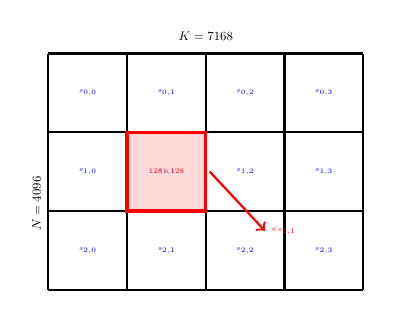
\begin{tikzpicture}[scale=0.5,transform shape]
  \draw[step=2,thick](0,0) grid (8,-6);
  \node[above,font=\small\bfseries] at (4,0.2){$K=7168$};
  \node[left,font=\small\bfseries,rotate=90] at (-0.3,-3){$N=4096$};
  \foreach \i in {0,...,3}{\foreach \j in {0,...,2}{
    \node[font=\tiny,blue] at (\i*2+1,-\j*2-1){$s_{\j,\i}$};}}
  \fill[red!25,opacity=0.6](2,-2) rectangle(4,-4);
  \draw[red,very thick](2,-2) rectangle(4,-4);
  \node[font=\tiny\bfseries,red] at(3,-3){$128{\times}128$};
  \draw[->,thick,red](4.1,-3)--(5.5,-4.5)
    node[right,font=\tiny]{$\times s_{1,1}$};
\end{tikzpicture}
\end{columns}
\end{frame}

%-----------------------------------------------------------
\begin{frame}{Concrete Example: Routing $T=4$ Tokens Through 3 Experts}
\small
\textbf{Setup:} 4 input tokens, 3 local experts (0,1,2), top-2 routing (simplified)

\medskip
\begin{columns}[T]
\column{0.48\textwidth}
\textbf{Step 1 --- Logits \& Routing}
\scriptsize
\begin{tabular}{c|ccc|cc}
\toprule
Token & $s_0$ & $s_1$ & $s_2$ & Top-2 & Weights \\
\midrule
$t_0$ & 0.9 & 0.2 & 0.7 & E0, E2 & 0.56, 0.44 \\
$t_1$ & 0.5 & 0.8 & 0.3 & E1, E0 & 0.62, 0.38 \\
$t_2$ & 0.3 & 0.6 & 0.9 & E2, E1 & 0.60, 0.40 \\
$t_3$ & 0.8 & 0.4 & 0.2 & E0, E1 & 0.67, 0.33 \\
\bottomrule
\end{tabular}

\bigskip
\textbf{Step 2 --- Dispatch Table}\\[2pt]
\scriptsize
\begin{tabular}{c|l}
\toprule
Expert & Tokens (weight) \\
\midrule
E0 & $t_0$ (0.56), $t_1$ (0.38), $t_3$ (0.67) \\
E1 & $t_1$ (0.62), $t_2$ (0.40), $t_3$ (0.33) \\
E2 & $t_0$ (0.44), $t_2$ (0.60) \\
\bottomrule
\end{tabular}

\column{0.50\textwidth}
\textbf{Step 3 --- Expert E0 computes ($T_k=3$)}
\scriptsize
\begin{enumerate}
  \item \textbf{Gather} rows $t_0, t_1, t_3$ from hidden states $\to A_e\ [3, 7168]$
  \item \textbf{GEMM1}: $A_e \cdot W_{1,0}^\top \to [3, 4096]$
  \begin{itemize}\scriptsize
    \item FP8 weights $\times$ block scales on-the-fly inside kernel
  \end{itemize}
  \item \textbf{SwiGLU}: split $[3,4096]$ into gate+up each $[3,2048]$
  \begin{itemize}\scriptsize
    \item $C = \text{gate} \odot \text{silu}(\text{up}) \to [3, 2048]$
  \end{itemize}
  \item \textbf{GEMM2}: $C \cdot W_{2,0}^\top \to [3, 7168]$
  \item \textbf{Scatter-add} with route weights:
  \begin{itemize}\scriptsize
    \item \texttt{accum}[$t_0$] $+=$ output$[0] \times 0.56$
    \item \texttt{accum}[$t_1$] $+=$ output$[1] \times 0.38$
    \item \texttt{accum}[$t_3$] $+=$ output$[2] \times 0.67$
  \end{itemize}
\end{enumerate}
Repeat for E1, E2. Final \texttt{accum} cast to BF16.
\end{columns}
\end{frame}

%-----------------------------------------------------------
\begin{frame}{Routing Detail: DeepSeek Grouped Top-K}
\small
\textbf{Why grouped?} 256 experts is large. Groups reduce search width while balancing load.

\medskip
\begin{columns}[T]
\column{0.52\textwidth}
\textbf{Step by step (per token):}
\begin{enumerate}\small
  \item $s = \sigma(\text{logits}) \in [0,1]^{256}$
  \item $s_b = s + \text{bias}_{256}$ \quad(load-balance nudge)
  \item Reshape to $[8\text{ groups},32\text{ experts}]$
  \item Score each group $=$ sum of top-2 experts in $s_b$
  \item Keep \textbf{top-4 groups} (128 survivors remain)
  \item From survivors, pick global \textbf{top-8 experts}
  \item Weights: $w_k = s[\text{idx}_k] / \sum s[\text{idx}] \times \alpha$
\end{enumerate}
\smallskip
\textbf{Critical:} use \emph{unbiased} $s$ for weights --- bias only guides selection.

\column{0.45\textwidth}
\begin{exampleblock}{\small Example (1 token, 8 groups)}
\scriptsize
\begin{tabular}{cl}
Group & Score (top-2 sum) \\
\hline
0 & 1.42 $\leftarrow$ selected \\
1 & 0.95 \\
2 & 1.31 $\leftarrow$ selected \\
3 & 1.18 $\leftarrow$ selected \\
4 & 0.72 \\
5 & 1.05 $\leftarrow$ selected \\
6 & 0.83 \\
7 & 0.91 \\
\end{tabular}
\vspace{2pt}

Groups 1,4,6,7 masked $\to -\infty$.\\
Top-8 picked from remaining 128.
\end{exampleblock}
\end{columns}
\end{frame}
